% THIS DOCUMENT FOLLOWS THE VOLERE TEMPLATE BY Suzanne Robertson and James Robertson
% ONLY THE SECTION HEADINGS ARE PROVIDED
%
% Updated Version Addressing Rubric Feedback
%
\documentclass[12pt]{article}

%-------------------------------------
% Packages
%-------------------------------------
\usepackage{booktabs}
\usepackage{tabularx}
\usepackage{longtable}
\usepackage{hyperref}
\usepackage{graphicx}

\hypersetup{
    bookmarks=true,         % show bookmarks bar?
    colorlinks=true,        % false: boxed links; true: colored links
    linkcolor=red,          % color of internal links (change box color with linkbordercolor)
    citecolor=green,        % color of links to bibliography
    filecolor=magenta,      % color of file links
    urlcolor=cyan           % color of external links
}

\newcommand{\lips}{\textit{Insert your content here.}}

%-------------------------------------
% Title, Author, and Date
%-------------------------------------
\title{Software Requirements Specification for MES-ERP}
\author{Group 26: MES Finance System}
\date{\today}

\begin{document}

\maketitle

\pagenumbering{roman}

\tableofcontents

\newpage

\section*{Revision History}
\begin{tabularx}{\textwidth}{p{3cm}p{2cm}X}
  \toprule
  \textbf{Date} & \textbf{Version} & \textbf{Notes} \\
  \midrule
  10/11/2024 & Revision 0 & Initial draft of SRS \\
  04/04/2025 & Revision 1 & 
    Added context diagrams, references, reflection, \\
    & & and traceability matrix. Revised section headings \\
    & & for clarity. Removed unnecessary tech constraints \\
    & & and addressed rubric feedback \\
  \bottomrule
\end{tabularx}

\newpage
\pagenumbering{arabic}

%-------------------------------------
% 1. Purpose of the Project
%-------------------------------------
\section{Purpose of the Project}
This section explains why the project exists and identifies the high-level goals or benefits that the solution will provide to the stakeholders.

\subsection{User Business}
The McMaster Engineering Society (MES) is seeking a platform that can streamline reimbursements for 60 student groups. Current manual methods (Google Forms, PDFs) result in lost requests, delayed payment, and limited oversight. A centralized, web-based solution will significantly reduce these issues.

\subsection{Goals of the Project}
\begin{itemize}
    \item \textbf{Reduce Wait Times and Lost Requests:} Provide rapid turnaround for reimbursements and mitigate the risk of losing requests.
    \item \textbf{Enhance Oversight:} Enable real-time tracking of budgets and transactions to keep clubs informed of their financial standing.
    \item \textbf{Improve User Experience:} Streamline the submission process with an intuitive interface and provide guidance where needed.
\end{itemize}

%-------------------------------------
% 2. System Overview
%-------------------------------------
\section{System Overview}
This section gives a high-level view of how the system operates and shows the major components.

\begin{figure}[h!]
  \centering
  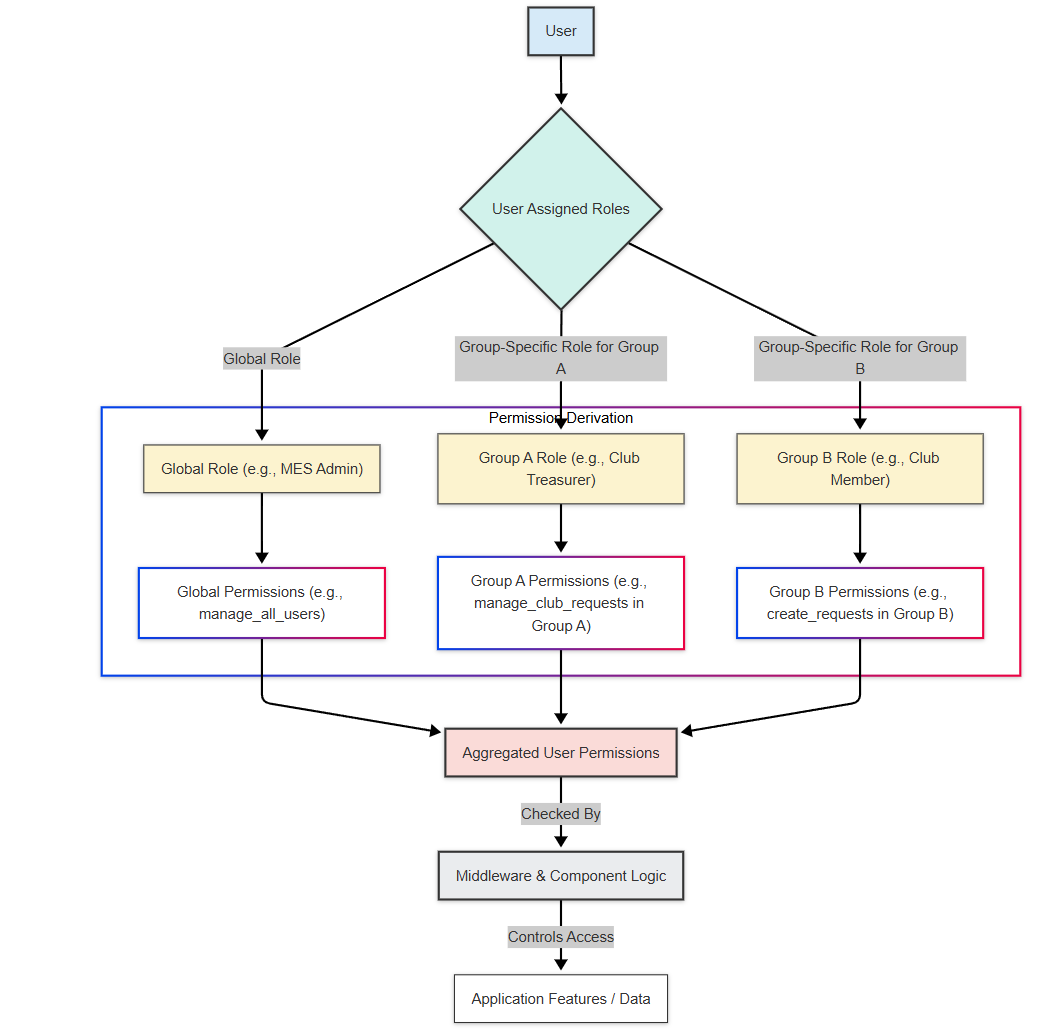
\includegraphics[width=0.9\textwidth]{system_detail.png}
  \caption{Context Diagram Showing Boundaries and User Interactions}
  \label{fig:detailed-architecture}
\end{figure}

The above diagram shows the main external actors (e.g., Club Financial Managers, Administrators) interacting with the system. Users submit requests, while administrators approve or reject them. The system stores all data in a secure database and sends notifications to keep everyone informed.

\begin{figure}[h!]
  \centering
  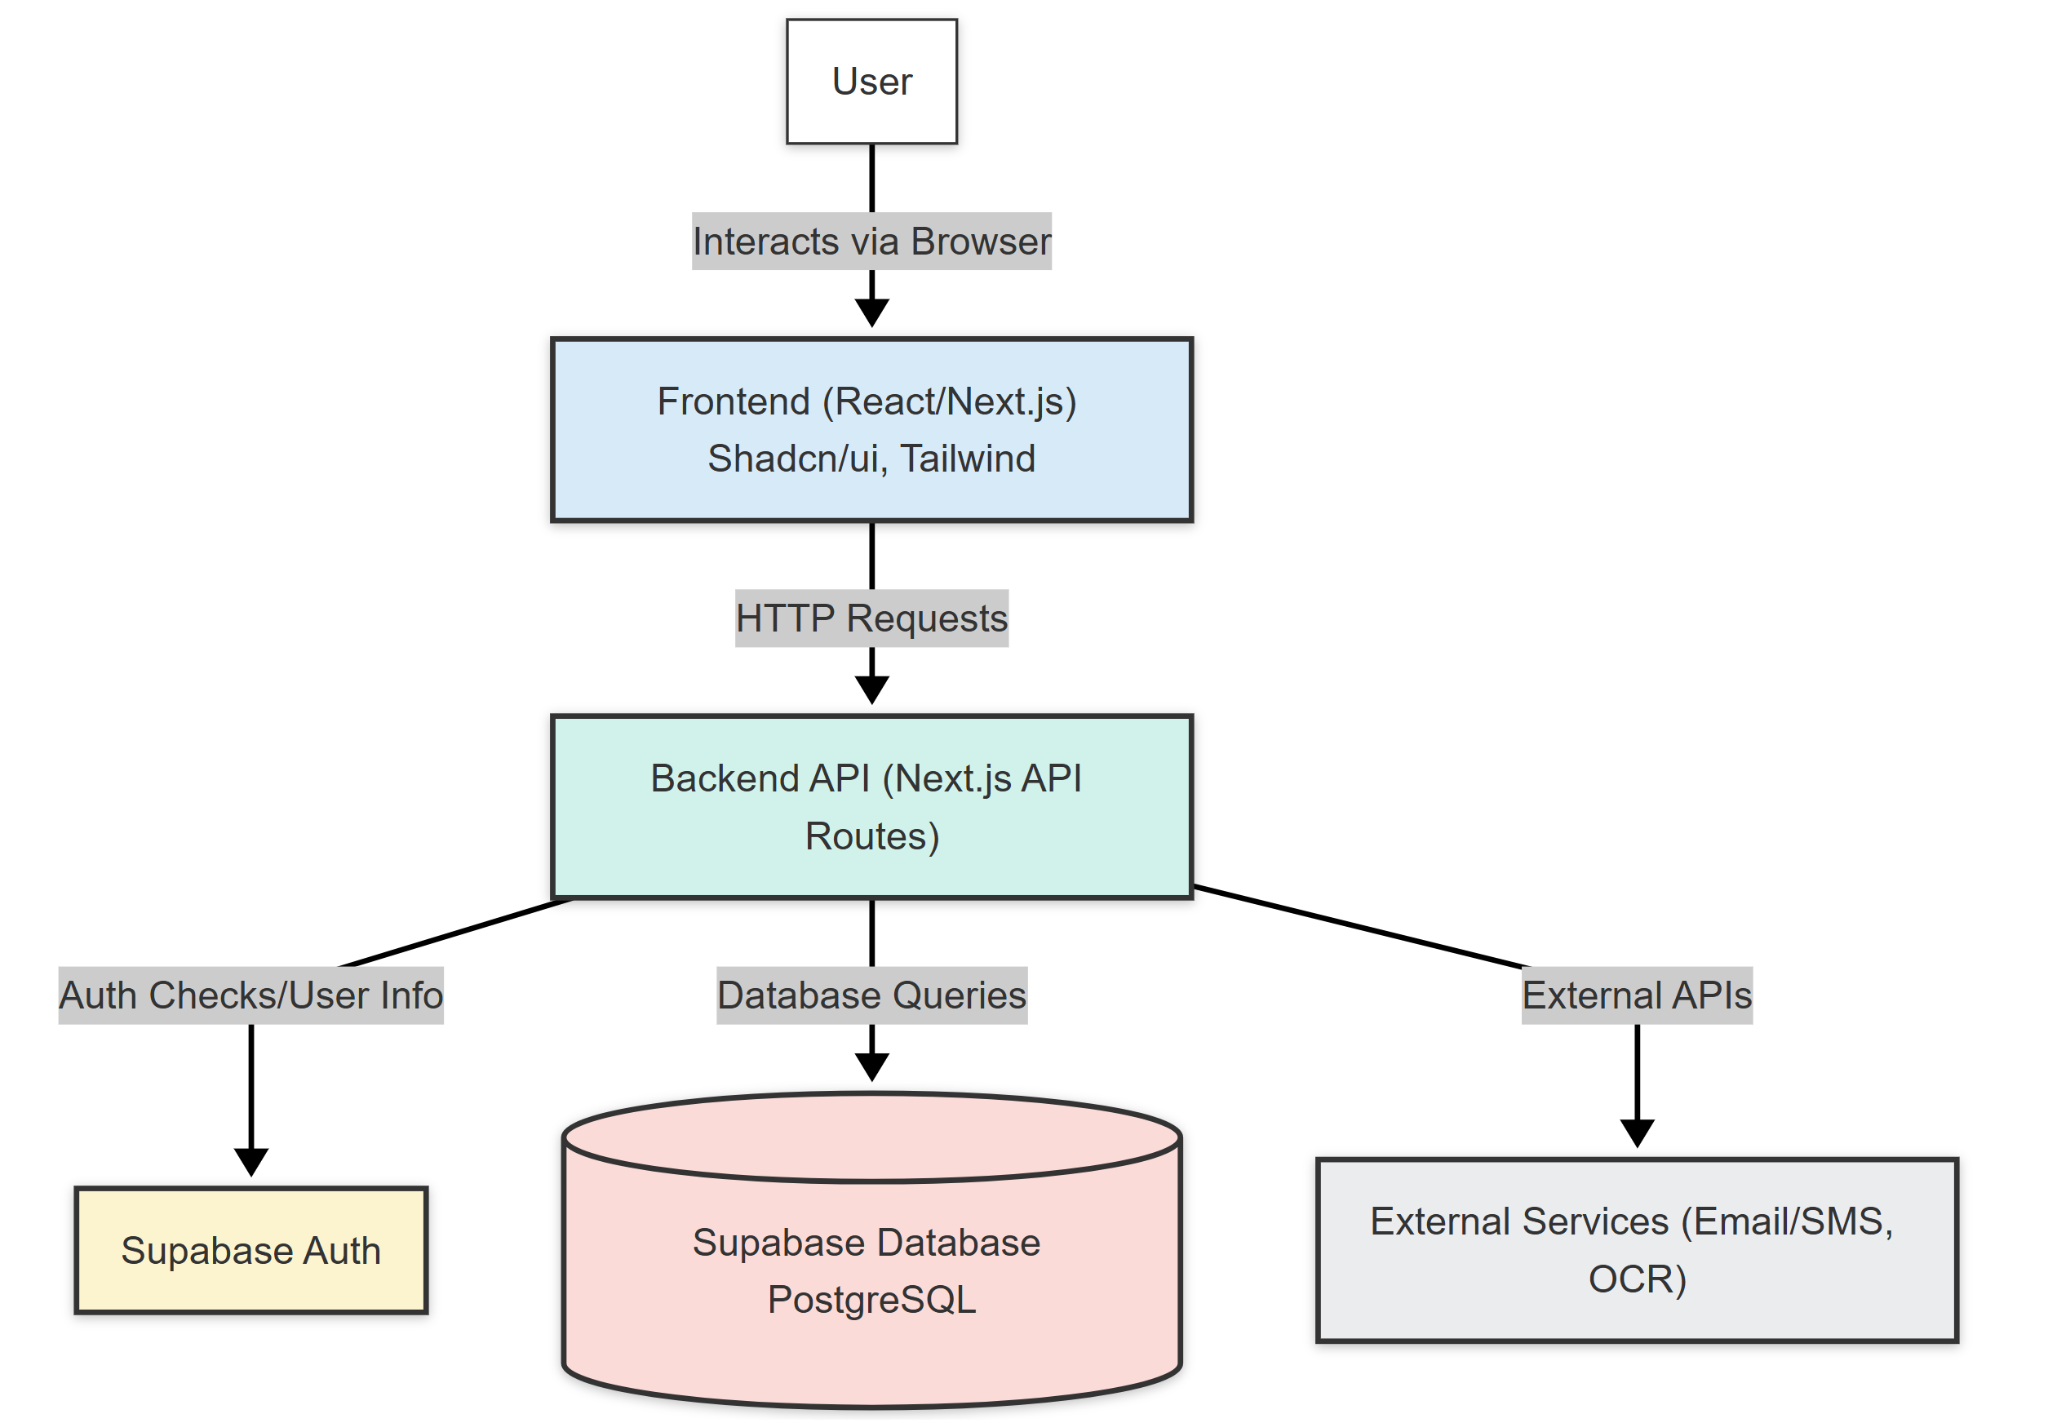
\includegraphics[width=0.9\textwidth]{stack.png}
  \caption{High-Level System Architecture (Logical View)}
  \label{fig:stack-architecture}
\end{figure}

The system is logically split into:
\begin{itemize}
    \item A front-end layer handling user interactions (forms, dashboards).
    \item A back-end layer managing business logic and communicating with the database.
\end{itemize}

%-------------------------------------
% 3. Stakeholders
%-------------------------------------
\section{Stakeholders}
This section identifies all persons or groups who have a stake in the project.

\subsection{Client}
\textbf{McMaster Engineering Society (MES)} -- invests in and approves the final product.

\subsection{Customer}
\begin{itemize}
    \item \textbf{Student Groups}: Use the system to request reimbursements.
    \item \textbf{MES Administrative Personnel}: Review and process incoming requests.
\end{itemize}

\subsection{Other Stakeholders}
\begin{itemize}
    \item \textbf{Student Group Leaders}
    \item \textbf{Club Members}
    \item \textbf{Financial Administrators}
    \item \textbf{McMaster Administration}
    \item \textbf{MES IT Team}
\end{itemize}

\subsection{Hands-On Users of the Project}
\begin{itemize}
    \item \textbf{Student Leaders}: Typically 18-25, manage club finances.
    \item \textbf{Administrators}: Approve or reject requests.
    \item \textbf{Financial Administrators}: Oversee advanced financial compliance and reporting.
\end{itemize}

\subsection{Personas}
\begin{itemize}
    \item \textbf{Alex, the Student Leader (20)}
    \item \textbf{Jamie, the MES Administrator (21)}
    \item \textbf{James, the VP Finance (22)}
    \item \textbf{Jordan, the Club Member (19)}
\end{itemize}

\subsection{User Participation}
\begin{itemize}
    \item \textbf{Requirements Gathering}: Interviews, surveys with user groups.
    \item \textbf{Usability Testing}: Hands-on sessions to validate design.
\end{itemize}

\subsection{Maintenance Users and Service Technicians}
\begin{itemize}
    \item \textbf{MES IT Staff}: Manage upgrades, address issues, monitor logs.
\end{itemize}

%-------------------------------------
% 4. Mandated Constraints
%-------------------------------------
\section{Mandated Constraints}
This section covers constraints imposed by stakeholders, technology, or external factors.

\subsection{Solution Constraints}
\begin{enumerate}
  \item Must manage reimbursement requests for 60 student groups.
  \item Must track and display the status of each request.
  \item Must allow attaching digital receipts (PDF or image).
  \item Must remain online consistently or provide an offline message.
\end{enumerate}

\subsection{Implementation Environment of the Current System}
\begin{enumerate}
  \item No existing digital system in place; everything is manual.
  \item The final system will be deployed on MES-owned infrastructure (minimum Windows 10, 4GB RAM).
\end{enumerate}

\subsection{Partner or Collaborative Applications}
\begin{enumerate}
  \item N/A
\end{enumerate}

\subsection{Off-the-Shelf Software}
\begin{enumerate}
  \item Third-party receipt scanning API may be integrated if feasible.
\end{enumerate}

\subsection{Anticipated Workplace Environment}
\begin{enumerate}
  \item Primarily an indoor environment with stable internet.
\end{enumerate}

\subsection{Schedule Constraints}
\begin{enumerate}
  \item The final demonstration is slated for April 2nd.
\end{enumerate}

\subsection{Budget Constraints}
\begin{enumerate}
  \item The project must stay within a \$750 budget.
\end{enumerate}

\subsection{Enterprise Constraints}
\begin{enumerate}
  \item All source code and documentation become MES property.
\end{enumerate}

%-------------------------------------
% 5. Naming Conventions and Terminology
%-------------------------------------
\section{Naming Conventions and Terminology}
Below is a glossary defining terms and acronyms to ensure clarity:

\begin{itemize}
    \item \textbf{MES}: McMaster Engineering Society
    \item \textbf{Audit Log}: Record of user actions and changes in the system
    \item \textbf{Budget Allocation}: Funding for specific clubs or events
    \item \textbf{Approval Workflow}: Path a request follows from submission to approval
    \item \textbf{Financial Dashboard}: Overview of budgets, reimbursements, and reports
    \item \textbf{CI/CD}: Continuous Integration/Continuous Deployment
\end{itemize}

%-------------------------------------
% 6. Relevant Facts And Assumptions
%-------------------------------------
\section{Relevant Facts And Assumptions}
This section discusses known facts and assumptions about the environment, users, and business rules.

\subsection{Relevant Facts}
\begin{itemize}
  \item Currently reliant on spreadsheets and manual PDF forms.
  \item The system must be easy to learn for student volunteers.
\end{itemize}

\subsection{Business Rules}
\begin{itemize}
  \item Users receive notifications upon reimbursement.
  \item All financial records must be maintained in the back end for audits.
\end{itemize}

\subsection{Assumptions}
\begin{itemize}
  \item MES provides the server and test data.
  \item Adequate internet connectivity for normal usage.
\end{itemize}

%-------------------------------------
% 7. The Scope of the Work
%-------------------------------------
\section{The Scope of the Work}
Here we describe the current situation, how our system fits into it, and how the project tasks are partitioned.

\subsection{The Current Situation}
Manual processing leads to lost submissions, slow approvals, and poor record-keeping.

\subsection{The Context of the Work}
Implementing a single platform to unify reimbursements, budget tracking, and reporting.

\subsection{Work Partitioning}
\begin{itemize}
  \item \textbf{Reimbursement Submission Module}
  \item \textbf{Reimbursement Review and Approval}
  \item \textbf{Audit and Compliance Module}
  \item \textbf{Budget/User Dashboards}
\end{itemize}

\subsection{Specifying a Business Use Case (BUC)}
\textbf{BUC 1: Submitting a Reimbursement Request}
\begin{itemize}
  \item \textit{Precondition}: Valid user credentials
  \item \textit{Steps}: User logs in, fills form, uploads receipt, submits
  \item \textit{Postcondition}: Request is logged as “pending approval”
\end{itemize}

%-------------------------------------
% 8. Business Data Model and Data Dictionary
%-------------------------------------
\section{Business Data Model and Data Dictionary}
This section details core data structures/entities and their relationships.

\subsection{Business Data Model}
\begin{itemize}
  \item \textbf{User Entity}: (UserID, Name, Email, Role, etc.)
  \item \textbf{Reimbursement Request Entity}: (RequestID, Timestamp, SubmitterID, Amount, Status, Receipts)
  \item \textbf{Budget Entity}: (BudgetID, GroupID, TotalAllocated, AmountSpent)
  \item \textbf{Group Entity}: (GroupID, GroupName, CreatedAt)
\end{itemize}

\subsection{Data Dictionary}
\textbf{N/A at this stage.} (No additional specialized terms to define beyond the glossary.)

%-------------------------------------
% 9. The Scope of the Product
%-------------------------------------
\section{The Scope of the Product}
This section distinguishes what the system will (and will not) do.

\subsection{Product Boundary}
\begin{itemize}
  \item \textbf{Automated Functions}: Online submission, notification sending, approval workflow
  \item \textbf{Manual Functions}: User training, legacy data entry from historical records
\end{itemize}

\subsection{Product Use Case Table}
\begin{table}[h]
  \centering
  \caption{Product Use Case (PUC) Summary}
  \begin{tabular}{|c|l|l|l|}
  \hline
   \textbf{PUC No} & \textbf{PUC Name} & \textbf{Actor/s} & \textbf{I/O} \\ \hline
   1 & Submit Reimbursement & Student Leader & In: expense data, receipts \\
     & & & Out: confirmation \\
   \hline
   2 & Review Requests & Administrator & In: pending requests \\
     & & & Out: approved/rejected \\
   \hline
   3 & Track Payment & Administrator & In: payment info \\
     & & & Out: payment status \\
   \hline
   4 & Process Funding App & Student Leader & In: application \\
     & & & Out: approval status \\
   \hline
   5 & Save User Data & Student Leader & In: user data \\
     & & & Out: data saved \\
   \hline
   6 & Send Notifications & System & In: event triggers \\
     & & & Out: emails/SMS \\
   \hline
   7 & Manage Audit Logs & Financial Auditor & In: filter criteria \\
     & & & Out: log reports \\
   \hline
  \end{tabular}
\end{table}

%-------------------------------------
% 10. Functional Requirements
%-------------------------------------
\section{Functional Requirements}
Below are the core functional requirements that define **what** the product must do, not **how** it will be done.

\begin{itemize}
  \item \textbf{FR-001}: The system must allow club financial managers (or authorized users) to submit reimbursement requests with attached receipts. \\
  \textbf{Rationale}: Essential to record expenses digitally. \\
  \textbf{Fit Criterion}:
    \begin{itemize}
      \item User with “Club Financial Manager” role can upload receipts and complete a reimbursement form.
      \item Request appears in system’s pending queue 95\% of the time without errors.
    \end{itemize}
  \textbf{Priority}: High

  \item \textbf{FR-002}: The system must allow MES staff to approve or reject reimbursement requests, updating status accordingly. \\
  \textbf{Rationale}: Needed for finalizing payments. \\
  \textbf{Fit Criterion}:
    \begin{itemize}
      \item Administrator can set a request’s status to Approved or Rejected.
      \item Update is visible to the submitter in under 2 seconds.
    \end{itemize}
  \textbf{Priority}: High

  \item \textbf{FR-003}: The system must notify request submitters of any status change in their reimbursement requests. \\
  \textbf{Rationale}: Submitters need real-time updates. \\
  \textbf{Fit Criterion}:
    \begin{itemize}
      \item Notifications (email or chosen method) dispatched within 30 seconds of status change.
      \item 90\% of notifications should reach users successfully under normal conditions.
    \end{itemize}
  \textbf{Priority}: Medium

  \item \textbf{FR-004}: The system must let administrators access financial records, audit logs, and user actions for compliance. \\
  \textbf{Rationale}: Complete oversight is necessary for audits and record-keeping. \\
  \textbf{Fit Criterion}:
    \begin{itemize}
      \item Administrator can retrieve any record or action log within 5 seconds.
      \item Logs are maintained for at least one year.
    \end{itemize}
  \textbf{Priority}: High
\end{itemize}

%-------------------------------------
% 11. Look and Feel Requirements
%-------------------------------------
\section{Look and Feel Requirements}
This section clarifies how the user interface should appear and what style/tone it should maintain.

\subsection{Appearance Requirements}
\begin{enumerate}
  \item Animations kept minimal and only for necessary feedback.
  \item Clear labeling of fields, with error states highlighted.
\end{enumerate}

\subsection{Style Requirements}
\begin{enumerate}
  \item No offensive imagery or language.
  \item Professional, formal tone.
  \item Consistent iconography and layout.
\end{enumerate}

%-------------------------------------
% 12. Usability and Humanity Requirements
%-------------------------------------
\section{Usability and Humanity Requirements}
Brief introduction: This section covers how easy it should be for people to learn, remember, and effectively use the system.

\subsection{Ease of Use Requirements}
\begin{enumerate}
  \item UI elements shall be consistent to help new users find features quickly.
  \item The system’s main features shall be reachable in \textbf{3 clicks or fewer}.
\end{enumerate}

\subsection{Accessibility Requirements}
\begin{enumerate}
  \item Offer a high-contrast mode for visually impaired users (AODA compliance).
  \item Provide textual alternatives for non-text content (icons, images).
\end{enumerate}

\subsection{Learning Requirements}
\begin{enumerate}
  \item Provide an optional tutorial overlay on first login.
\end{enumerate}

%-------------------------------------
% 13. Performance Requirements
%-------------------------------------
\section{Performance Requirements}
**Introduction**: Performance covers speed, capacity, and fault-tolerance. Below are the key parameters to ensure the system remains responsive under normal and peak loads.

\subsection{Speed and Latency Requirements}
\begin{itemize}
    \item 90\% of page loads under 2 seconds under typical usage.
    \item Form submission for reimbursements under 2 seconds for normal conditions.
\end{itemize}

\subsection{Safety-Critical Requirements}
\begin{itemize}
  \item N/A (No life-critical functionality).
\end{itemize}

\subsection{Precision or Accuracy Requirements}
\begin{itemize}
    \item Monetary values displayed with exactly 2 decimal places.
\end{itemize}

\subsection{Robustness or Fault-Tolerance Requirements}
\begin{itemize}
    \item Daily backups of data to prevent catastrophic loss.
\end{itemize}

\subsection{Capacity Requirements}
\begin{itemize}
    \item Support at least 200 concurrent users without major slowdown.
\end{itemize}

\subsection{Scalability or Extensibility Requirements}
\begin{itemize}
    \item Adding new user roles or groups shall not require major schema changes.
\end{itemize}

\subsection{Longevity Requirements}
\begin{itemize}
    \item Maintainable for at least 5 years with moderate developer effort.
\end{itemize}

%-------------------------------------
% 14. Operational and Environmental Requirements
%-------------------------------------
\section{Operational and Environmental Requirements}
Short introduction: This section identifies how and where the system operates, including OS/hardware constraints and neighboring systems.

\subsection{Expected Physical Environment}
\begin{enumerate}
  \item Office/lab environments with stable power/network connections.
\end{enumerate}

\subsection{Wider Environment Requirements}
\begin{enumerate}
  \item Replaces existing paper/Google Forms approach.
\end{enumerate}

\subsection{Requirements for Interfacing with Adjacent Systems}
\begin{enumerate}
  \item Must be usable on Windows, Mac, and Linux, with major modern browsers.
\end{enumerate}

\subsection{Productization Requirements}
\begin{enumerate}
  \item N/A (Internal deployment only).
\end{enumerate}

\subsection{Release Requirements}
\begin{enumerate}
  \item Perform regression tests before each new release.
\end{enumerate}

%-------------------------------------
% 15. Maintainability and Support Requirements
%-------------------------------------
\section{Maintainability and Support Requirements}
Short introduction: This section covers how the system can be maintained and supported over its life cycle.

\subsection{Maintenance Requirements}
\begin{enumerate}
  \item Future expansions for more clubs or advanced features should not require total rework.
\end{enumerate}

\subsection{Supportability Requirements}
\begin{enumerate}
  \item Must run on MES-authorized devices with at least Windows 10 and 4GB RAM.
\end{enumerate}

\subsection{Adaptability Requirements}
\begin{enumerate}
  \item Must handle scaling to 100 clubs as the MES grows.
\end{enumerate}

%-------------------------------------
% 16. Security Requirements
%-------------------------------------
\section{Security Requirements}
Brief introduction: Addresses protection of data, user privacy, and logging/auditing.

\subsection{Access Requirements}
\begin{enumerate}
  \item Administrators have full privileges; club managers see only their own data.
\end{enumerate}

\subsection{Integrity Requirements}
\begin{enumerate}
  \item Changes to financial data must be logged with user ID, timestamp, and action.
\end{enumerate}

\subsection{Privacy Requirements}
\begin{enumerate}
  \item Comply with PIPEDA, ensuring user consent and data minimization.
\end{enumerate}

\subsection{Audit Requirements}
\begin{enumerate}
  \item Exportable logs of all financial actions must be available to auditors.
\end{enumerate}

\subsection{Immunity Requirements}
\begin{enumerate}
  \item Third-party libraries used must be reviewed monthly for security updates.
\end{enumerate}

%-------------------------------------
% 17. Cultural Requirements
%-------------------------------------
\section{Cultural Requirements}
\begin{enumerate}
  \item Default interface in English (British spelling if needed).
  \item Use inclusive, neutral language.
\end{enumerate}

%-------------------------------------
% 18. Compliance Requirements
%-------------------------------------
\section{Compliance Requirements}
\subsection{Legal Requirements}
\begin{itemize}
    \item Must follow PIPEDA for data handling.
    \item Must meet AODA guidelines for accessibility in Ontario.
\end{itemize}

\subsection{Standards Compliance Requirements}
\begin{itemize}
    \item Aim to follow ISO/IEC 27001 guidelines on information security.
    \item Adhere to agile software development principles.
\end{itemize}

%-------------------------------------
% 19. Open Issues
%-------------------------------------
\section{Open Issues}
\begin{itemize}
  \item \textbf{Issue \#001}: Notification method (email vs.\ SMS vs.\ in-app) is still to be decided.
  \item \textbf{Issue \#002}: Retention period for logs remains undefined; possibly 1--2 years or more.
  \item \textbf{Issue \#003}: Thresholds for multiple approval levels (if any) are not finalized.
\end{itemize}

%-------------------------------------
% 20. Off-the-Shelf Solutions
%-------------------------------------
\section{Off-the-Shelf Solutions}
\subsection{Ready-Made Products}
\begin{enumerate}
  \item N/A (No direct off-the-shelf product matches MES’s exact requirements).
\end{enumerate}

\subsection{Reusable Components}
\begin{enumerate}
  \item Potential use of common UI libraries or receipt-scanning APIs.
\end{enumerate}

\subsection{Products That Can Be Copied}
\begin{enumerate}
  \item Inspiration from existing budgeting/expense-tracking apps but no direct copy due to custom MES needs.
\end{enumerate}

%-------------------------------------
% 21. New Problems
%-------------------------------------
\section{New Problems}
\subsection{Effects on the Current Environment}
\begin{itemize}
    \item Training required for staff and volunteers new to the system.
\end{itemize}

\subsection{Effects on Installed Systems}
\begin{itemize}
    \item Potential integration with existing MES financial spreadsheets or data exports.
\end{itemize}

\subsection{Potential User Problems}
\begin{itemize}
    \item Resistance to replacing manual processes.
\end{itemize}

\subsection{Limitations in the Anticipated Implementation Environment}
\begin{itemize}
    \item Limited hardware resources or network outages could disrupt usage.
\end{itemize}

\subsection{Follow-Up Problems}
\begin{itemize}
    \item Additional training needed if advanced features are introduced later.
\end{itemize}

%-------------------------------------
% 22. Tasks
%-------------------------------------
\section{Tasks}
\subsection{Project Planning}
An agile approach (e.g., Scrum) with iterative sprints and stakeholder check-ins every 1--4 weeks.

\subsection{Planning of the Development Phases}
\begin{longtable}{| m{3cm} | m{10cm} |}
  \hline
  \textbf{Step} & \textbf{Description} \\
  \hline
  Requirements Gathering & Interviews, feedback from MES staff and club managers \\
  \hline
  Sprint Planning & Estimation and prioritization using a backlog \\
  \hline
  Design \& Architecture & Establish data models, system design, refine prototypes \\
  \hline
  Development & Implement features in short cycles (1--4 weeks each) \\
  \hline
  Testing & Continuous integration, unit + integration + acceptance tests \\
  \hline
  Review \& Retrospective & Evaluate progress, collect stakeholder feedback \\
  \hline
  Release & Deploy stable increments, ensure regression tests are passed \\
  \hline
\end{longtable}

\subsection{Requirement Priority}
\begin{itemize}
    \item \textbf{High Priority}: Functional Reqs (FR-001, FR-002, FR-004), Security/Privacy, Compliance
    \item \textbf{Medium Priority}: Performance, Usability/Accessibility, Maintainability
    \item \textbf{Low Priority}: Minor UI aesthetics (as long as they do not hamper usability)
\end{itemize}

%-------------------------------------
% 23. Migration to the New Product
%-------------------------------------
\section{Migration to the New Product}
\subsection{Requirements for Migration}
\begin{itemize}
  \item N/A (No mandatory migration from previous database; legacy data remains in spreadsheets unless decided otherwise).
\end{itemize}

\subsection{Data Modification or Translation}
\begin{itemize}
  \item N/A (No forced data migration on day 1).
\end{itemize}

%-------------------------------------
% 24. Costs
%-------------------------------------
\section{Costs}
\subsection{Labor Costs}
\begin{itemize}
  \item 400--500 hrs dev, 50--70 hrs testing (approx.)
\end{itemize}

\subsection{Monetary Costs}
\begin{itemize}
  \item Server electricity, minor hardware upgrades: \$10--\$20/month
\end{itemize}

\subsection{Additional Considerations}
\begin{itemize}
  \item Maintenance: 5--10 hrs/month post-launch
\end{itemize}

%-------------------------------------
% 25. Likely Changes
%-------------------------------------
\section{Likely Changes}
\begin{enumerate}
  \item Adding a mobile app for capturing receipts.
  \item Advanced analytics or ML-based tagging of expenses.
  \item Support for more robust multi-approval workflows if MES finances grow.
\end{enumerate}

%-------------------------------------
% 26. Ideas for Solution
%-------------------------------------
\section{Ideas for Solution}
A responsive, web-based finance tool with:
\begin{itemize}
  \item A front-end framework (e.g., React) for the UI.
  \item A back-end capable of storing requests and logs securely in a relational DB.
  \item CI/CD pipeline to allow frequent and safe deployments.
\end{itemize}

%-------------------------------------
% 27. Requirements Traceability
%-------------------------------------
\section{Requirements Traceability}
This matrix shows how each Functional Requirement (FR) ties back to the Product Use Cases (PUCs) defined earlier, ensuring coverage and clarity.

\begin{table}[h]
  \centering
  \caption{Traceability Matrix: FRs to PUCs}
  \begin{tabular}{|c|c|l|}
    \hline
    \textbf{FR \#} & \textbf{PUC \#} & \textbf{Description/Notes} \\
    \hline
    FR-001 & PUC 1 & Submitting Reimbursement Request \\
    \hline
    FR-002 & PUC 2 & Approving/Rejecting Requests \\
    \hline
    FR-003 & PUC 1,2,6 & Status changes require notifications \\
    \hline
    FR-004 & PUC 7 & Admin oversight and audit logs \\
    \hline
  \end{tabular}
\end{table}

By maintaining this table, we ensure each requirement is testable against specific use cases, and no requirement is orphaned or redundant.

%-------------------------------------
% References
%-------------------------------------
\section*{References}
\begin{flushleft}
Hunter, C. (n.d.). \textit{Software Requirements Specification (SRS)} [PDF]. GitHub.  
\url{https://github.com/cer-hunter/OAR-CAS741/blob/main/docs/SRS/SRS.pdf}

\medskip

McMaster Engineering Society. (n.d.). \textit{Home}.  
\url{https://macengsociety.ca/}
\end{flushleft}

%-------------------------------------
% Appendix - Reflection
%-------------------------------------
\section*{Appendix --- Reflection}
This section is used to evaluate the team on the graduate attribute of Lifelong Learning.  

\begin{enumerate}
  \item \textbf{What knowledge and skills will the team collectively need?} \\
  We will need:
  \begin{itemize}
    \item \textbf{Financial Workflow Knowledge}: Understanding MES reimbursement, budgeting cycles, etc.
    \item \textbf{UI/UX Design}: Building easy-to-use interfaces.
    \item \textbf{Backend/Data Management}: Handling secure and scalable data storage.
    \item \textbf{Agile Project Management}: Sprints, retros, backlog grooming, etc.
  \end{itemize}

  \item \textbf{Approaches to acquiring or mastering these skills:} \\
  \begin{itemize}
    \item \textbf{Domain Knowledge}: Direct interviews with MES finance staff; analyzing existing documents.
    \item \textbf{UI/UX}: Iterative prototyping; collecting user feedback.
    \item \textbf{Backend/Data}: Tutorials, official documentation, proof-of-concept builds.
    \item \textbf{Project Management}: Use of GitHub Projects or similar tool; active communication with the team.
  \end{itemize}
\end{enumerate}

\end{document}